\graphicspath{{./images/}}

\newcounter{nonFuncReq} %Non functinal requiremet counter
\newcounter{quatar} %Quality target counter

\chapter{Einführung und Ziele}

\section{Business Case}
\label{businesscase}

Die Applikation MEON dient der Registration neuer Händler für den mobilen Bezahldienst Paymit (Twint aktuell nicht klar) und zukünftig der Registrierung neuer Händler für Enabling(Terminal)/Acquiring Pakete.  Der Geschäftsprozess ist in der folgenden Grafik vereinfacht dargestellt:

\textcolor{red}{/* TODO als ersten Schritt würde ich sowas wie "Merchant fills registration data" einführen, oder Start On-Boarding genauer erklären */}
\begin{center}
	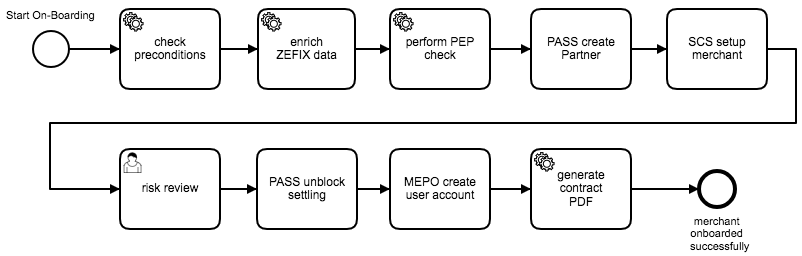
\includegraphics[scale=0.4]{meon-workflow.png}
\end{center}

Die folgende Tabelle beschreibt die einzelnen Teile des Prozesses genauer.

\begin{table}[H]
	\centering
	\caption{Prozessteile}
	\begin{tabular}{ | p{4cm} | p{12cm} | }
		\toprule
		{\textbf{Name}} & {\textbf{Beschreibung}} \\
		\midrule
		Merchant fills registrations data & Der Händler füllt alle notwendigen Daten aus für den Vetrag aus \\ \hline
		Check preconditions & Überprüft Vorbedingungen wie techniusche Gültigkeit der Daten \textcolor{red}{/* TODO  hier bin ich nicht mehr sicher was alles überprüft wird} */ \\ \hline
		enrich ZEFIX data & Reichert die erhaltenen Daten mit dem Handelsregisterauszug an \\ \hline
		perform PEP Check & Prüft ob die Person politisch exponiert ist. \\ \hline
		PASS create partner & Erstellt den Händler (Partner) im Acquiring System.\\ \hline
		SCS setup merchant & Registriert den Händler im Enabling System für die Zahlungsterminals \\ \hline
		risk review  & Risiko Abschätzung im Fall einer politisch exponierten Person und Abklärung, ob ein risikotechnisch gültiger Geschäftsbereich vorliegt \\ \hline
	    PASS Unblock settling & Schaltet die Auszahlung der verarbeiteten Transaktionen im Acquiring System frei \\ \hline
	    MEPO create user account&  Erstellt einen Account im Kundenportal \\ \hline
	    generate contract PDF & Generiert ein ausgefülltes Vertrags-PDF und schickt es per E-Mail an den Händler \textcolor{red}{/* TODO Bei Paymit wurde der Vertrag nicht mehr unterschrieben */}  \\
		\bottomrule
	\end{tabular}
\end{table}

\section{Aufgabenstellung}

Die Architektur der Applikation MEON soll so angepasst werden das Continuous Deployment möglich wird. Damit ist gemeint das jeder Teil der Applikation eigenständig ausgerollt werden kann, ohne andere Komponenten herunterzufahren. Des Weiteren darf der Benutzer nicht von der Änderung beeinflusst sein respektive seine Anfragen dürfen durch ein Anheben einer Komponente nicht verloren gehen.
Die Paymit Onboarding Anwendung ist funktional komplett implementiert und keine weiteren Anforderungen sind bekannt. Neue funktionale Anforderungen müssen die hier erarbeitete Lösung miteinbeziehen, so dass das Continuous Deployment nicht beeinträchtigt wird.
Die Aufgabe besteht darin die Teile hinsichtlich der Kommunikation voneinander zu entkoppeln, so dass eine Aktualisierung den darin abgebildeten Geschäftsprozess nicht unterbricht.  Der interne Aufbau der Komponenten soll nur falls nötig angepasst werden. Die Benutzeroberfläche sowie deren Benutzbarkeit ist nicht Teil der Aufgabe.

\section{Anforderungen}

Alle funktionalen Anforderungen sind bereits umgesetzt. Durch die Anpassung der Architektur in Richtung Continuous Deployment gibt es aktuell nur nicht funktionale Anforderungen.

\begin{table}[H]
	\centering
	\caption{Nicht funktionale Anforderungen}
	\begin{tabular}{ | p{2cm} | p{14cm} | }
		\toprule
		{\textbf{ID}} & {\textbf{Beschreibung}} \\
		\midrule
		NFA-\arabic{nonFuncReq} \stepcounter{nonFuncReq} & Kunde merkt nicht wenn neue Komponenten der Applikation ausgetauscht werden. \\ \hline
		NFA-\arabic{nonFuncReq} \stepcounter{nonFuncReq} & Verfügbarkeit der Frontend-Anwendung ist 24x7 (SLA). \\ \hline
		NFA-\arabic{nonFuncReq} \stepcounter{nonFuncReq} & Einhaltung der PCI DSS Anforderung bezüglich Umgang mit Daten resp. deren Zugriffsschutz durch Authentifizierung, Authorisierung und entsprechende Netzwerksegmentierung. \\ \hline
		NFA-\arabic{nonFuncReq} \stepcounter{nonFuncReq} & Die Applikation muss einfach skalierbar sein. \\ \hline
		NFA-\arabic{nonFuncReq} \stepcounter{nonFuncReq} & Die Anwendung muss eine hohe Ausfallsicherheit für Server und die Datenbank aufweisen. \\ \hline
		NFA-\arabic{nonFuncReq} \stepcounter{nonFuncReq} & Bugfixing geschieht mittels vorwärts committen, anstelle von Hotfixes wird immer die ganze Applikation neu ausgerollt. \\ \hline
		NFA-\arabic{nonFuncReq} \stepcounter{nonFuncReq} & Die Anwendung lässt sich voll automatisch Ausrollen. \\ \hline
		NFA-\arabic{nonFuncReq} \stepcounter{nonFuncReq} & Konfigurationsänderungen an der Applikation sind ohne Neustart möglich.\\
		\bottomrule
	\end{tabular}
\end{table}

\subsection{Aspekte}

Die wichtigstens Aspekte der Fachdomäne sind: 
\begin{itemize}
	\item Auswahl eines Paymit Abos
	\item Vertragsabschluss
\end{itemize}

\subsection{Art des Systems}

Bei MEON handelt es sich um ein interaktives Onlinesystem.

\subsection{Nutzung des Systems}

\subsection{Schnittstellen}

MEON hat folgende Schnittstellen zu Umsystemen. \textcolor{red}{/* TODO ro = ReadOnly, w = Write, ev. nicht wichtig hier */}
\begin{itemize}
	\item AddressService: Adressen Service der Post (ro)
	\item UID: Schweizer Unternehmens-Identifikationsnummer (ro) 
	\item ZEFIX: Handelsregsiteranbindung (ro)
	\item PEP: Service zur Überprüfung politisch exponierter Personen (ro)
	\item ATMS: SMS Service (w)
	\item Email: Email Service (w)
	\item Workflow: Workflow Engine Backoffice SIX (w)
	\subitem PASS: Transaktionsverarbeitungssystem (w)
	\subitem SCS:  Verwaltung der Terminal geräte bei den Kunden (w)
\end{itemize}

\subsection{Datenhaltung}

\begin{itemize}
	\item RDBMS (Presistenz)
\end{itemize}

\section{Qualitätsziele}

Die folgende Tabelle zeigt die wichtigsten Qualitätsziele. Die Szenarien zu den Zielen sind genauer im Kapitel \ref{sec:qualityscenarios} aufgeführt.

\begin{table}[H]
	\centering
	\caption{Qualitätsziele}
	\begin{tabular}{ | p{3cm} | p{13cm} | }
		\toprule
		{\textbf{Name}} & {\textbf{Beschreibung}} \\
		\midrule
		Q-\arabic{quatar} \stepcounter{quatar} & Die neue Architektur soll einfach verständlich und anwendbar sein.\\ \hline
		Q-\arabic{quatar} \stepcounter{quatar} & Die Deployment Pipeline soll einfach wartbar sein. \\ \hline
		Q-\arabic{quatar} \stepcounter{quatar} & Der Benutzer wird durch eine Ausrollung der Anwendung nicht beeinträchtigt. \\ \hline
		Q-\arabic{quatar} \stepcounter{quatar} & Die Performanz wird durch eine Ausrollung der Applikation nicht beeinträchtigt.\\ 
		\bottomrule
	\end{tabular}
\end{table}

\section{Stakeholder}

\begin{table}[H]
	\centering
	\caption{Stakeholder}
	\begin{tabular}{ | p{3cm} | p{13cm} | }
		\toprule
		{\textbf{Name}} & {\textbf{Beschreibung}} \\
		\midrule
		Business & Repräsentiert die Geschäftstätigkeit der Firma.\\ \hline
		Kunde & Benutzer der Webapplikation. \\ \hline
		Support-Kunde & Support welcher den Kunden bei Problemen unterstützt. \\ \hline
		Legal &  Verantwortlich für die Richtigkeit der Vertragsabschlüsse. \\ \hline
		Risk & Sorgt für die Überprüfung der Personen und der Geschäftstätigkeiten. \\ \hline
		Marketing & Abteilung für den Vertrieb, Werbung, Design. \\ \hline
		Betrieb & Betreibt die Webapplikation auf der Infrastruktur der SIX \\ \hline
		Change Management & Genehmigt Änderungen an der Applikation. \\ \hline
		Entwickler & Setzt die Anforderungen der einzelnen Stakeholder um. \\
		\bottomrule
	\end{tabular}
\end{table}
